\apendice{Documentación de usuario}
En esta sección del anexo se han definido aquellos requisitos necesarios para la ejecución y puesta en marcha del proyecto. 
\section{Requisitos software y hardware para ejecutar el proyecto.}
\subsection{Requisitos del software}
Para el correcto funcionamiento es necesario tener instalado en el ordenador todas las herramientas y programas que se han utilizado. 
\begin{itemize}
    \item Python: Este programa es esencial para que el código se ejecute y se abra el desplegable.
    \item Arduino IDE: Este programa es necesario para tener una comunicación y conexión correcta entre la placa de arduino y el ordenador.
    \item Editor de texto/código: No es estrictamente necesario la instalación de un editor de texto/código como Visual Studio Code, pero sí puede facilitar el uso tanto al usuario como a posibles profesionales ingenieros para la solución de errores.
    \item Instalación de bibliotecas:
    \begin{itemize}
        \item Pandas: manipulación y análisis de datos estructurados(tablas).
        \item Pyserial: comunicación con puerto serie.
        \item Kivy: paquete que permite la creación de la interfaz gráfica
        \item kivymd: paquete que permite la creación de la interfaz gráfica
        \item Openpyxl: abrir y modificar archivos Excel.
        \item Cryptography: encriptar y desencriptar documentos, crea una clave para generar un cifrado simétrico.
    \end{itemize}

\begin{table}[]
\centering
\begin{tabular}{|l|l|}
\hline
\rowcolor[HTML]{BFBFBF} 
\textbf{Software} & \textbf{Descripción} \\ \hline
Python & Versión 3.13\\ \hline
Arduino IDE & Versión 2.3.6\\ \hline
Bibliotecas & Versiones más actualizadas\\ \hline
\end{tabular}
\caption{Requisitos Software}
\label{tab:Requisitos_Software}
\end{table}
\end{itemize}
\subsection{Requisitos del hardware}
Para el correcto funcionamiento es necesario el uso del dispositivo creado, un ordenador y el cable USB que conecte el ordenador con la placa de Arduino.
\section{Instalación / Puesta en marcha}
\subsection{Python}

El proceso de descargar Python es sencillo. Desde la web oficial de Python \cite{Python}, en la pantalla inicial (ver \textit{Figura} \ref{fig:Python}), aparece un botón de descarga (señalado con una flecha roja). Al seleccionarlo, la descarga se inicia de forma automática. Una vez descargado el archivo, el proceso de instalación se realiza de una forma similar a la de otras aplicaciones: se decide la ruta de instalación deseada y el programa queda instalado en nuestro ordenador.

\begin{figure}[h]
        \centering
        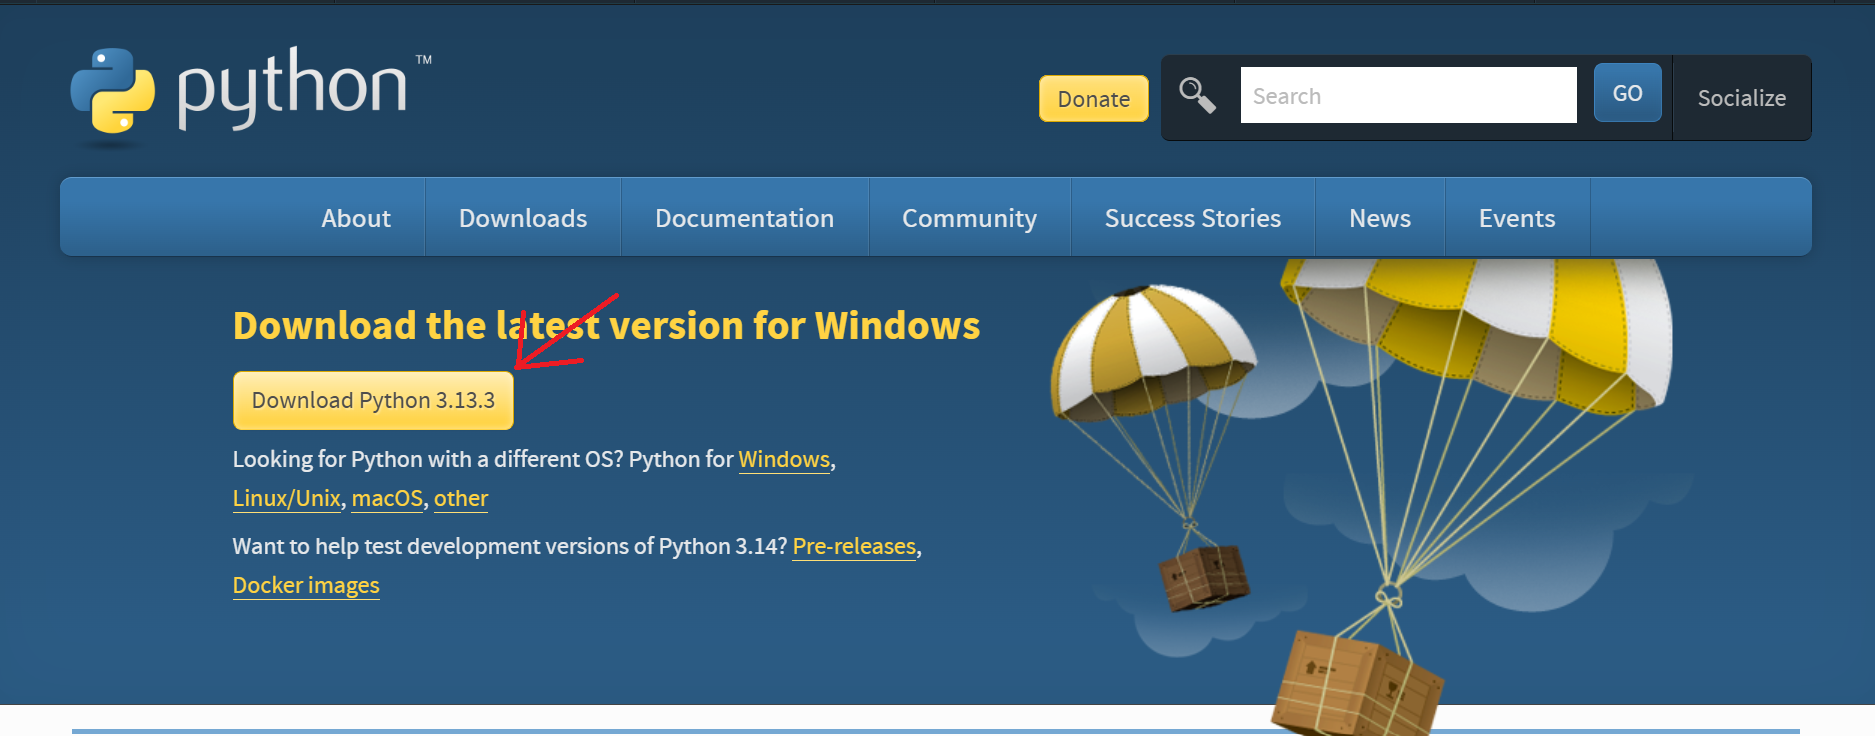
\includegraphics[width=0.8\textwidth]{img/pantalla inicio python.png}
        \caption{Pantalla descargar Python. Fuente python.org}
        \label{fig:Python}
    \end{figure}
\subsection{Arduino IDE}
Proceso muy similar a la instalación de Python. Desde la web oficial de Arduino IDE \cite{Arduino}, en la pantalla inicial (ver \textit{Figura} \ref{fig:Arduino}), aparece una sección de diferentes opciones de descarga según el sistema operativo instalado en el ordenador. Al seleccionar el archivo correspondiente a nuestro sistema operativo, se abre una ventana nueva en la cual hay que clicar el botón 'Just Download' y la descarga se iniciará de forma automática. Una vez descargado el archivo, el proceso de instalación se realiza de una forma similar a la de otras aplicaciones: se decide la ruta de instalación deseada y el programa queda instalado en nuestro ordenador.
    \begin{figure}[h]
        \centering
        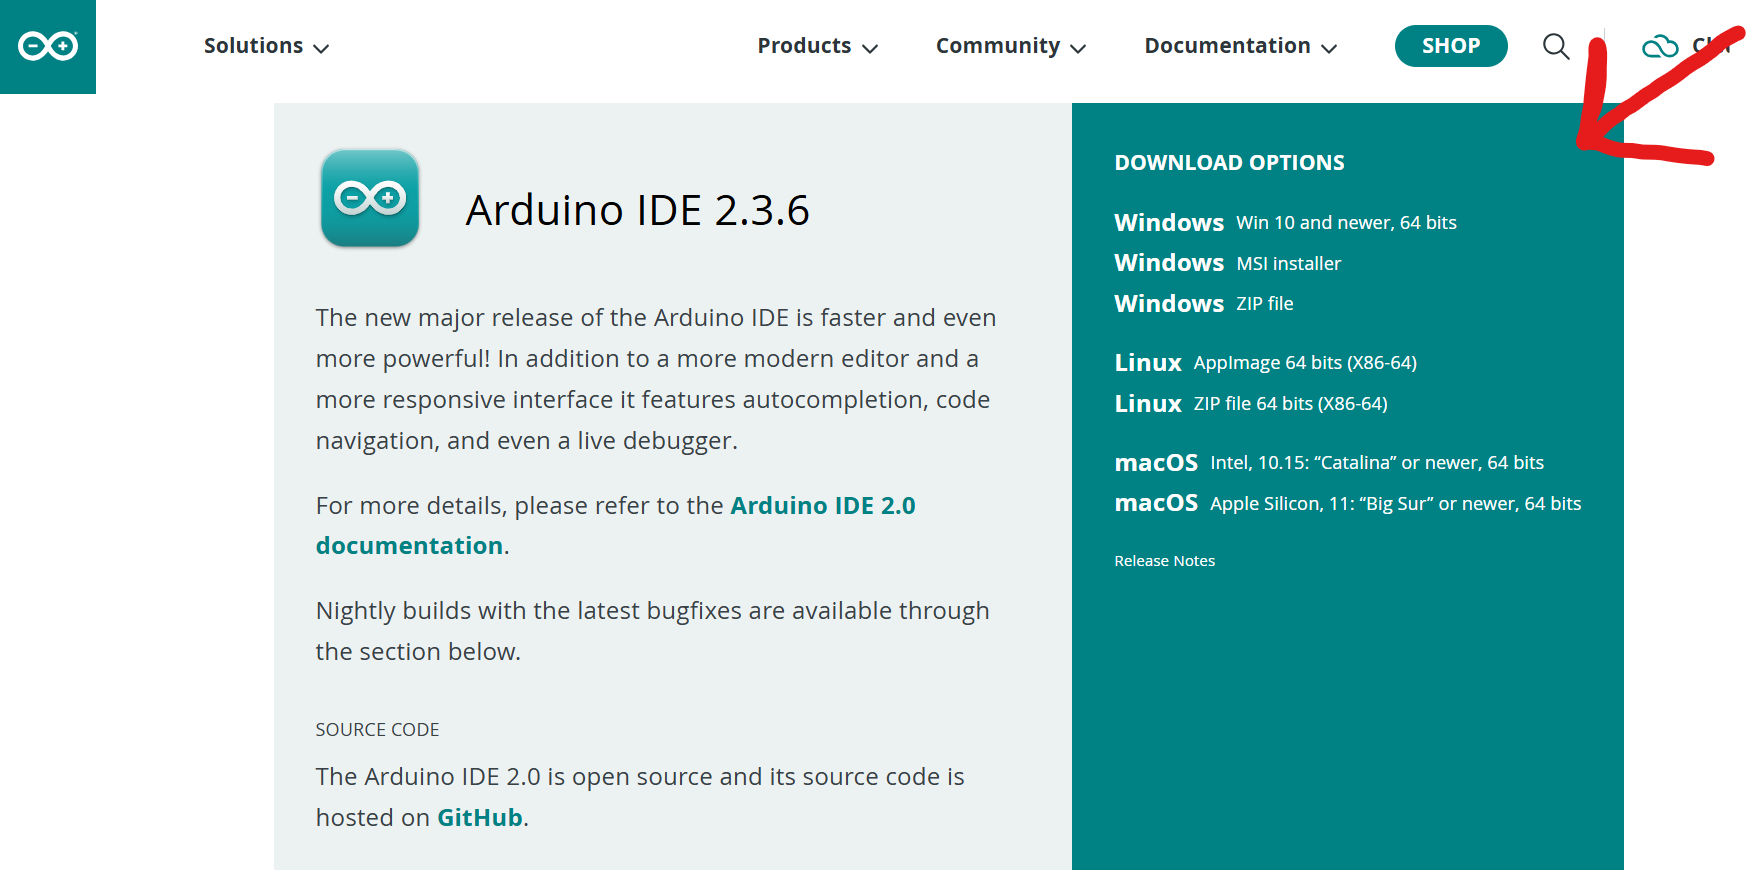
\includegraphics[width=1\textwidth]{img/pantalla inicio arduino IDE.png}
        \caption{Pantalla descargar Arduino. Fuente arduino.cc}
        \label{fig:Arduino}
    \end{figure}
\subsection{Instalación de bibliotecas}
La instalación de las bibliotecas se hace desde la consola del sistema (CMD). Para abrirla, basta con buscar CMD en el buscador de Windows y hacer clic sobre el resultado.
Una vez abierta la consola (ver \textit{Figura} \ref{fig:CMD}), se deben introducir los siguientes comandos para la instalación de las bibliotecas:
\begin{itemize}
    \item pip install pandas
    \item pip install pyserial
    \item pip install kivy 
    \item pip install kivymd
    \item pip install openpyxl
    \item pip install cryptography
\end{itemize}

\begin{figure}[h]
    \centering
    \includegraphics[width=0.8\textwidth]{img/pantalla CMD.png}
    \caption{Pantalla CMD. Fuente Propia}
    \label{fig:CMD}
\end{figure}

\subsection{Prototipo}
Para la puesta en marcha del prototipo físico, es necesario la correcta colocación de todos los componentes y mandar el código a la placa de forma correcta. 

En la \textit{Figura} \ref{fig:Vista esquemática prototipo}, se puede observar un esquema del prototipo físico.
\begin{figure}
    \centering
    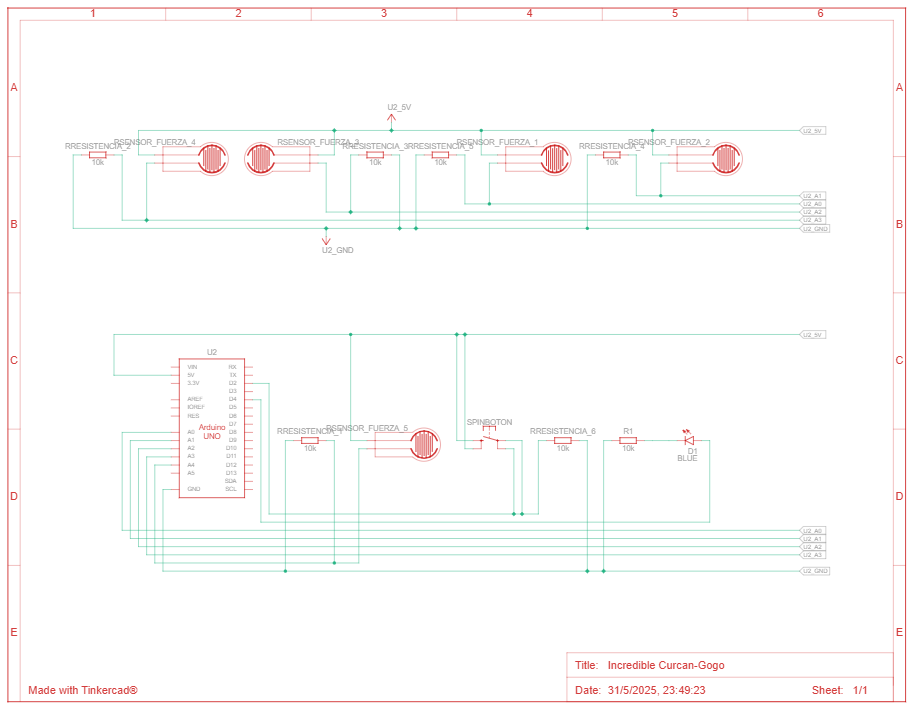
\includegraphics[width=1\linewidth]{img/Vista esquematica prototipo.png}
    \caption{Vista esquemática prototipo. Fuente propia}
    \label{fig:Vista esquemática prototipo}
\end{figure}
En las \textit{Figuras} \ref{fig:CodigoArduino1} \ref{fig:CodigoArduino2} \ref{fig:CodigoArduino3}, en orden se puede observar el código necesario para el correcto funcionamiento.
\begin{figure}
    \centering
    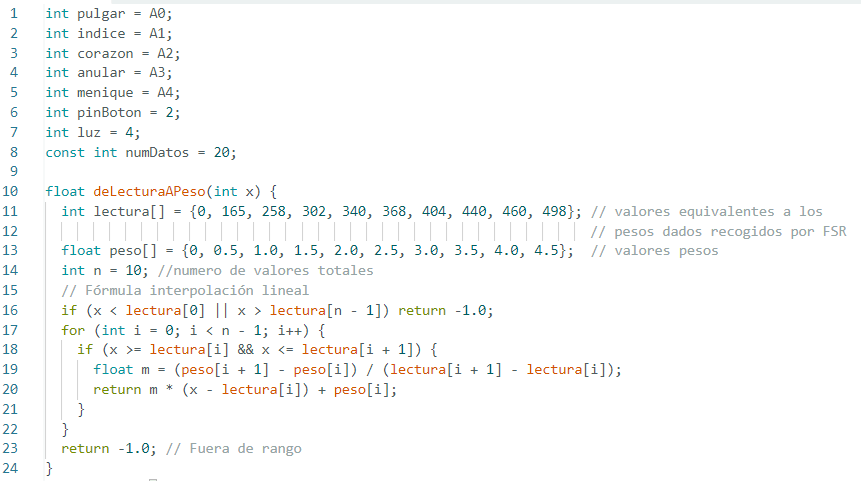
\includegraphics[width=1.25\linewidth]{img/CodigoArduino1.png}
    \caption{Código Arduino para el prototipo físico. Fuente propia}
    \label{fig:CodigoArduino1}
\end{figure}
\begin{figure}
    \centering
    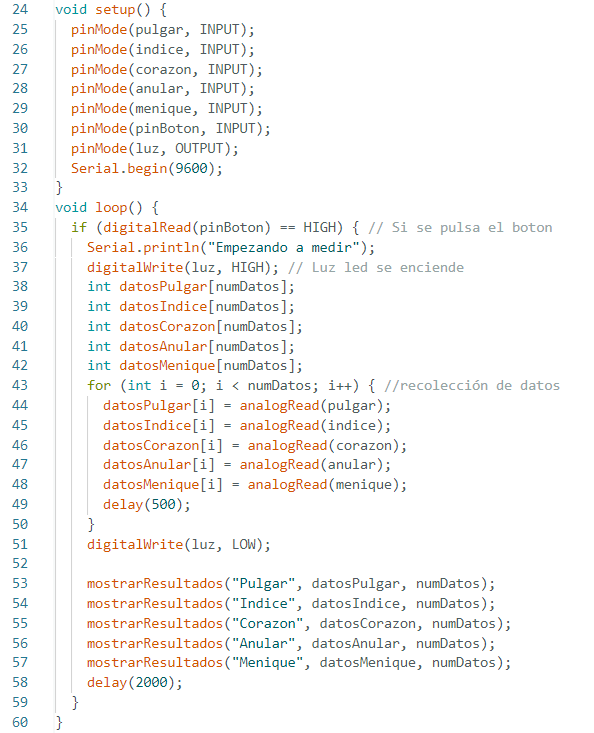
\includegraphics[width=1\linewidth]{img/CodigoArduino2.png}
    \caption{Código Arduino para el prototipo físico. Fuente propia}
    \label{fig:CodigoArduino2}
\end{figure}
\begin{figure}
    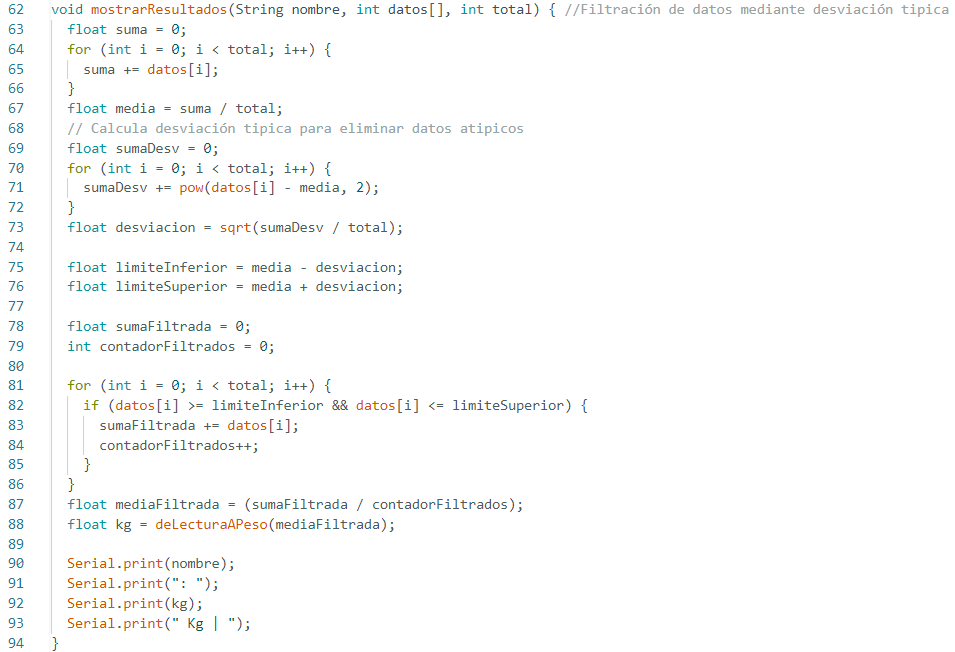
\includegraphics[width=1.25\linewidth]{img/CodigoArduino3.png}
    \caption{Código Arduino para el prototipo físico. Fuente propia}
    \label{fig:CodigoArduino3}
\end{figure}
\section{Manuales y/o Demostraciones prácticas}  

El dispositivo desarrollado en este proyecto se puede utilizar de maneras diferentes según la aplicación que se le quiera dar. A continuación, se va a realizar una demostración práctica del dispositivo sin ningún tipo de accesorio complementario. 

En primer lugar, se debe abrir el prototipo de la interfaz desarrollada (véase \textit{Figura} \ref{fig:Pantalla principal}). Si ya se dispone de una cuenta, se debe iniciar sesión; en caso contrario, es obligatorio crear una cuenta nueva y a continuación acceder iniciando sesión.

 \begin{figure}
        \centering
        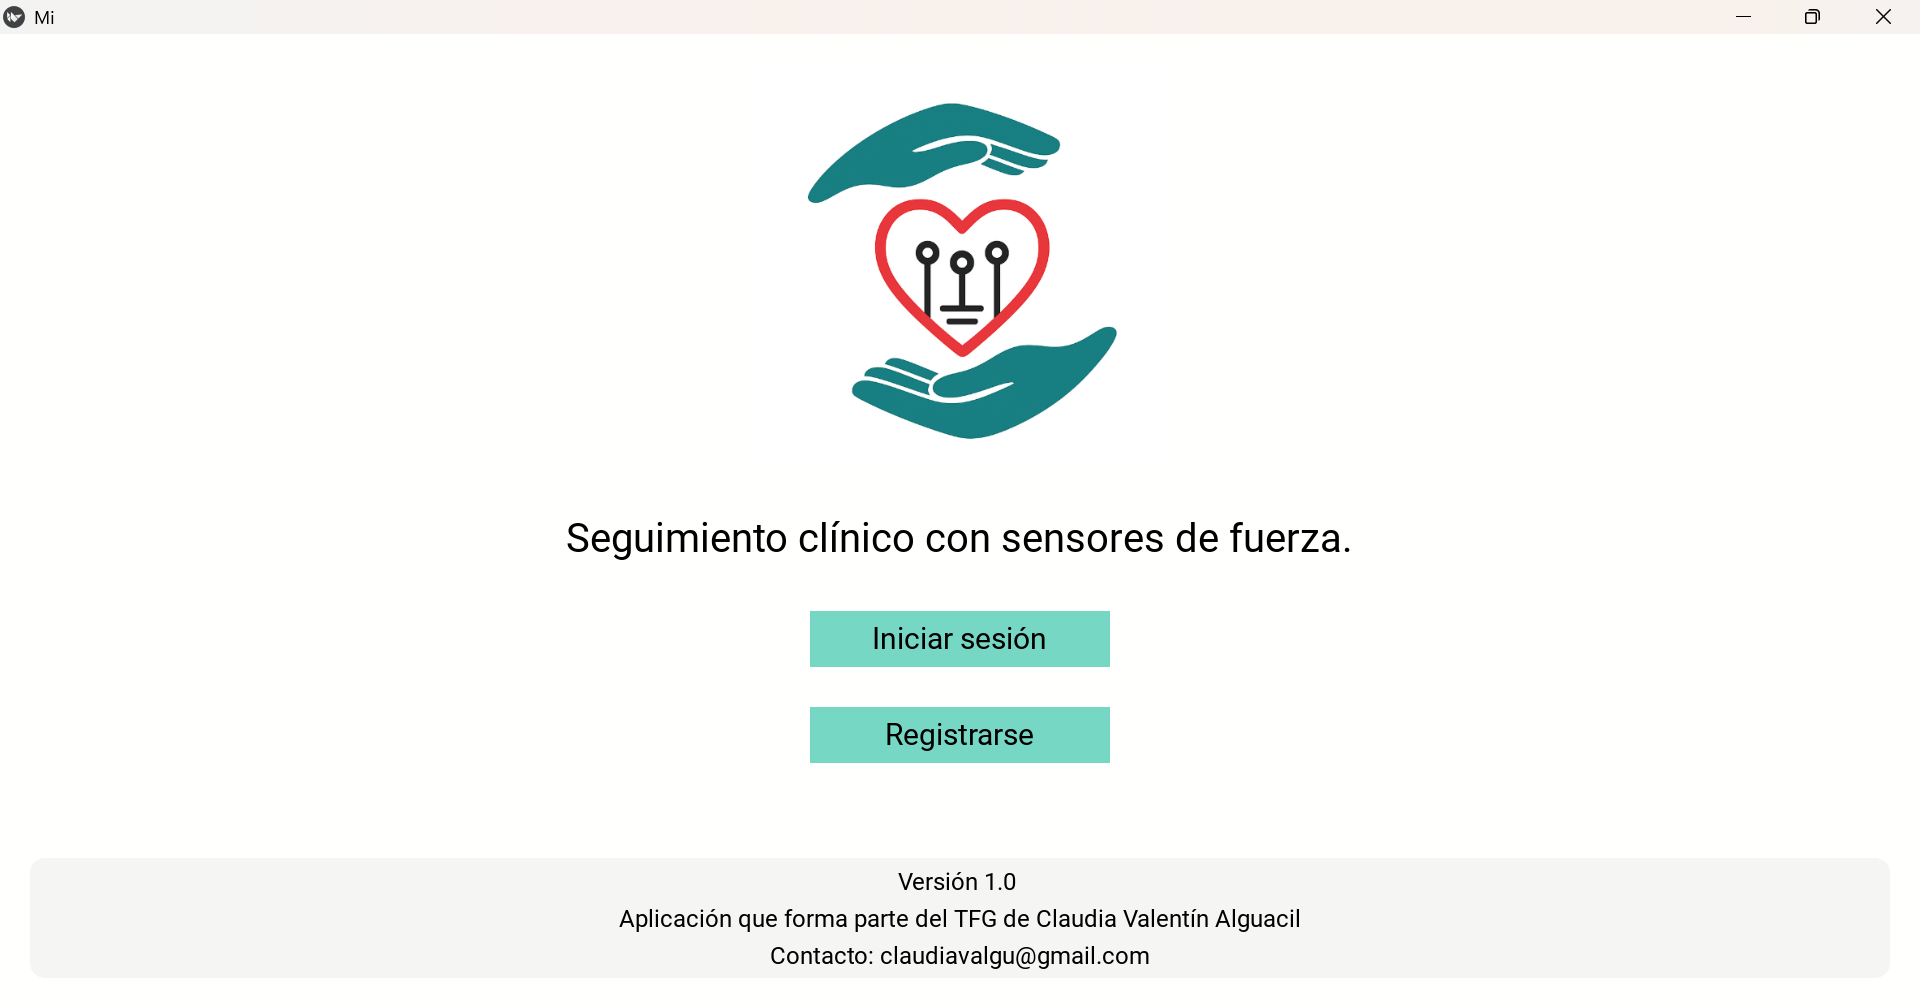
\includegraphics[width=1\linewidth]{img/Pantalla principal.png}
        \caption{Pantalla principal. Fuente Propia.}
        \label{fig:Pantalla principal}
\end{figure}

Una vez dentro, existen dos opciones, seleccionar un paciente ya registrado o bien añadir uno nuevo. Elegido o registrado el paciente, el usuario podrá elegir entre registrar una nueva medición o consultar las mediciones previamente almacenadas.

En caso de seleccionar la opción de registrar una nueva medición, se debe conectar la placa Arduino al puerto USB del ordenador. Una vez conectada, es necesario colocar los sensores sobre una superficie dura y estable (véase \textit{Figura} \ref{fig:sensores_mesa}), asegurando así la precisión de la lectura, colocar los dedos sobre cada sensor teniendo en cuenta la colorimetría de los cables: rojo-pulgar, naranja-índice, amarillo-corazón, verde-anular, marrón-meñique (véase \textit{Figura} \ref{fig:sensor_mano}). A continuación, se debe presionar el botón “Iniciar medición” en la interfaz y, seguidamente, pulsar el botón físico de la placa arduino, lo que dará inicio al proceso de medición. Durante este proceso, se encenderá una luz Led (véase \textit{Figura} \ref{fig:luz}) que indica que el dispositivo está recolectando los datos.
\begin{figure}
    \centering
    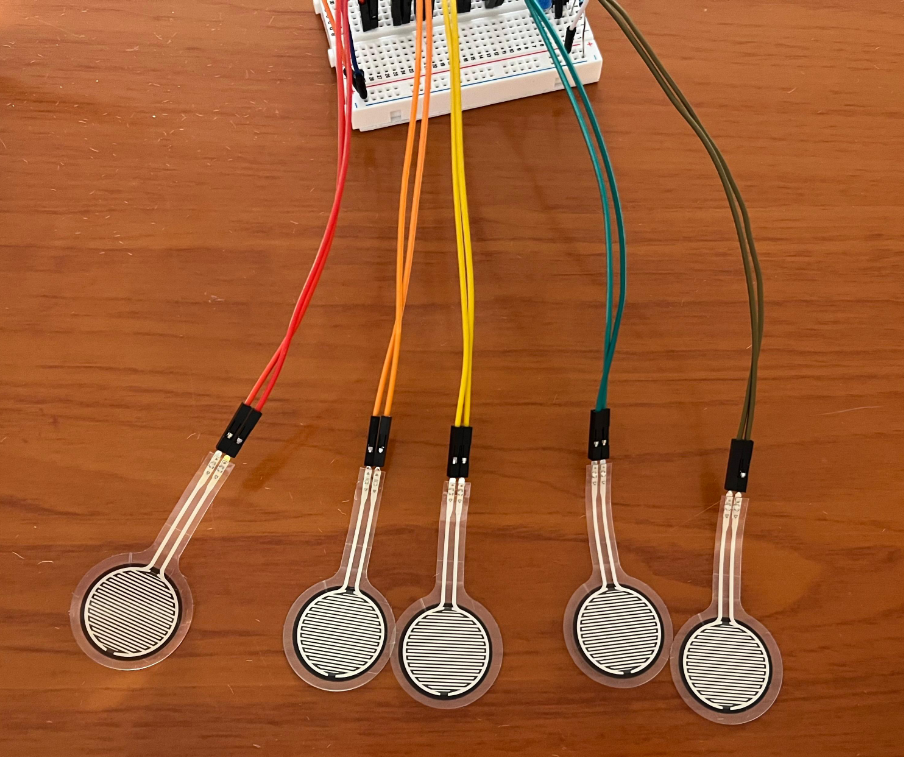
\includegraphics[width=0.5\linewidth]{img/Sensores.png}
    \caption{Sensores. Fuente propia}
    \label{fig:sensores_mesa}
\end{figure}
\begin{figure}
    \centering
    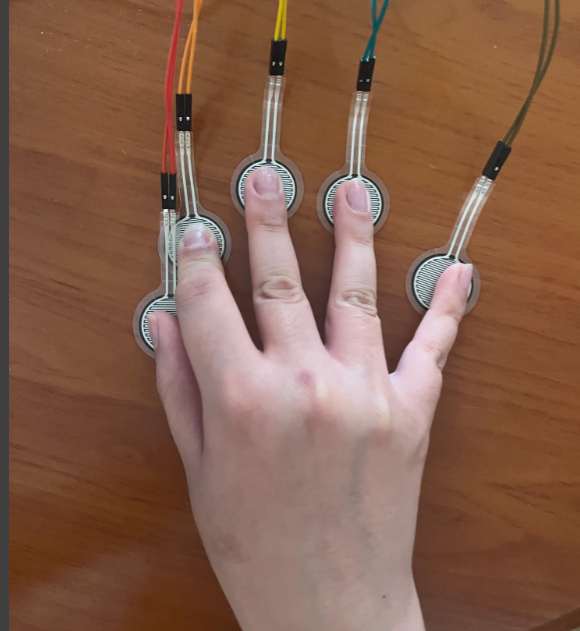
\includegraphics[width=0.5\linewidth]{img/sensor_mano.png}
    \caption{Disposición de los dedos en los sensores. Fuente propia}
    \label{fig:sensor_mano}
\end{figure}
\begin{figure}
    \centering
    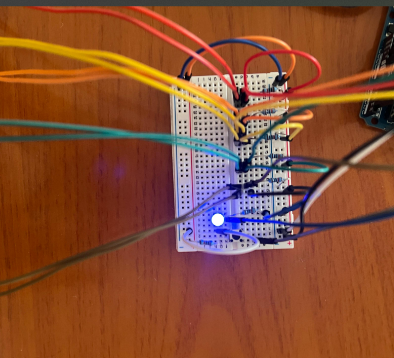
\includegraphics[angle=90 ,width=0.5\linewidth]{img/Luz_encendido.png}
    \caption{Luz led se enciende al empezar a recoger datos. Fuente propia}
    \label{fig:luz}
\end{figure}

Cuando el Led se apague, la medición habrá finalizado. Los resultados se podrán visualizar en la interfaz, ya sea de forma gráfica o numérica, seleccionando los botones correspondientes de “Visualización gráfica” o “Visualización registro”.

En la \textit{Figura} \ref{fig:Grafico} y en la \textit{Figura} \ref{fig:registro} se puede observar un registro realizado ejerciendo diferentes presiones a los sensores. 
\begin{figure}
    \centering
    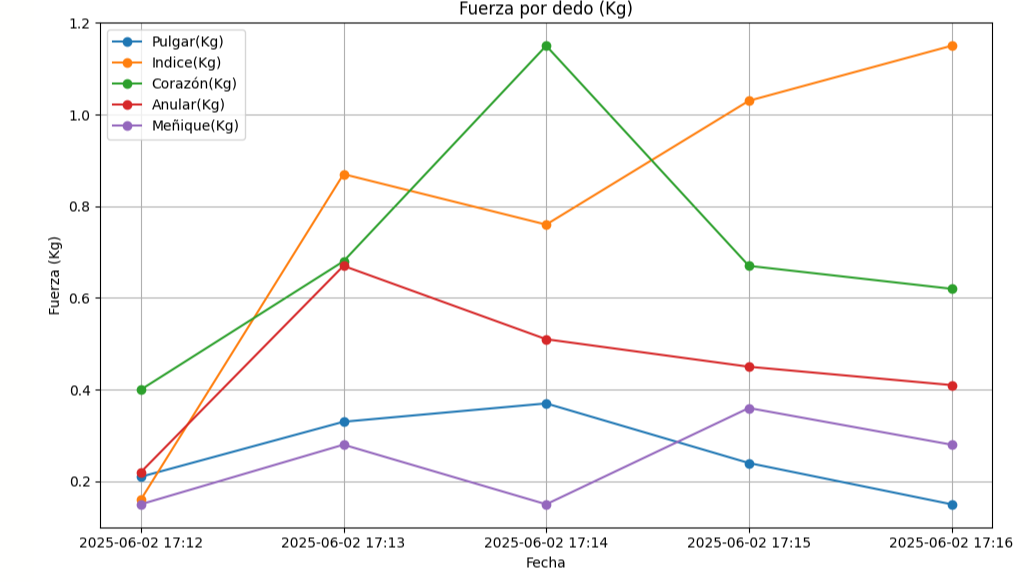
\includegraphics[width=1\linewidth]{img/grafica_fuerza.png}
    \caption{Gráfica de los datos recogidos. Fuente propia}
    \label{fig:Grafico}
\end{figure}

\begin{figure}
    \centering
    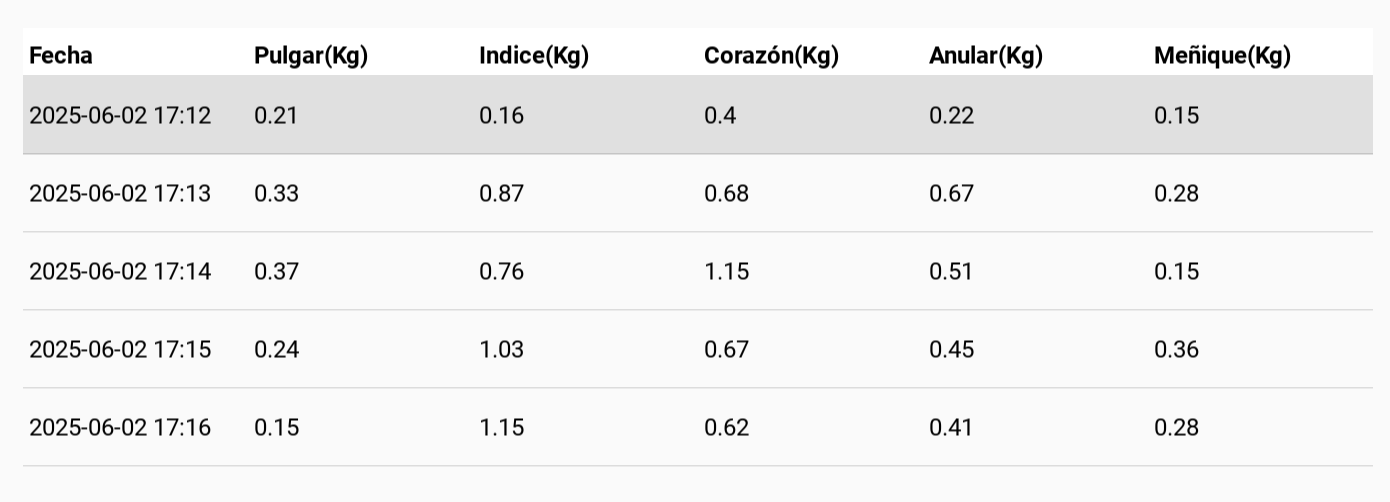
\includegraphics[width=1\linewidth]{img/Datos_medidas.png}
    \caption{Tabla de los datos recogidos. Fuente propia}
    \label{fig:registro}
\end{figure}